\documentclass{beamer}
% October 2016 
% Author: Dr Rachid Hourizi and Dr. Michael Wright 
% Department of Computer Science, University of Bath
\usepackage{listings}
\usetheme{Boadilla} 
\lstset{language=c,
	basicstyle=\ttfamily\small,
           keywordstyle=\color{blue}\ttfamily,
           stringstyle=\color{red}\ttfamily,
           commentstyle=\color{green}\ttfamily,
          breaklines=true}

\begin{document}

\AtBeginSection[]{
  \begin{frame}
  \vfill
  \centering
  \begin{beamercolorbox}[sep=8pt,center,shadow=true,rounded=true]{title}
    \usebeamerfont{title}\insertsectionhead\par%
  \end{beamercolorbox}
  \vfill
  \end{frame}
}

\title{CM10227/ CM50258: Lecture 5}
\author{Dr Rachid Hourizi and Dr. Michael Wright}
\date{\today}
\frame{\titlepage}

\begin{frame}
\frametitle{Housekeeping}
\begin{itemize}
\item We will post the first large Coursework on Moodle tomorrow (Friday)
\item Everyone must complete this coursework (CM10227 and CM50258)
\item It describes a considerably larger (Java) task than the lab sheet exercises
\item Take an Iterative development approach 
\begin{itemize}
\item Start with a program that does very little
\item Make sure that it works
\item Add functionality incrementally
\item Compiling and testing as you go
\end{itemize}
\item Dont leave it to the last minute (Hand in = 24th Nov)
\item Do remember that help is available in all the usual places
\end{itemize}
\end{frame}

\begin{frame}
\frametitle{Back to Java}
\begin{itemize}
\item Java forces us to 
\begin{itemize}
\item \textbf{define} a combination of data and operations once (a \alert{Class})
\item and then \textbf{create} one or more examples (instances) of that class (\alert{Objects})
\end{itemize}
\end{itemize}
\end{frame}

\begin{frame}
\frametitle{Review}
\begin{itemize}
\item Class bodies contain fields, constructors and methods.
\item Fields store values that determine an object’s state.
\item Constructors initialize objects.
\item Methods implement the behaviour of objects.
\begin{itemize}
\item Mutators (mutator methods) change the state of a object
\item Accessors (accessor methods) provide information about the state of an object 
\end{itemize}
\end{itemize}
\end{frame}

\begin{frame}
\frametitle{Review}
\begin{itemize}
\item Objects can make decisions via conditional (if) statements.
\item A true or false test allows one of two alternative courses of action to be taken.
\end{itemize}
\end{frame}

\section{Interacting Objects}

\begin{frame}
\frametitle{Developping Interactive Classes: A digital clock}
\begin{center}
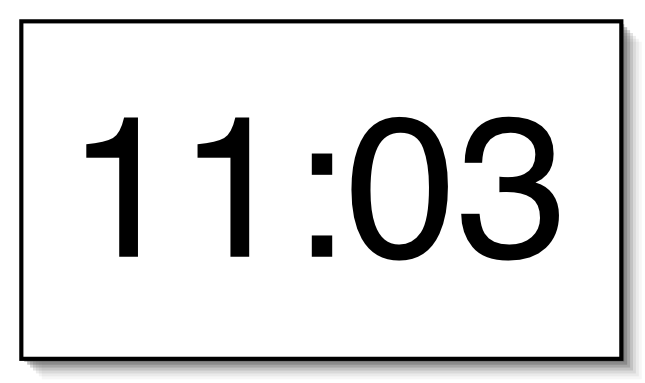
\includegraphics[height=5cm,keepaspectratio]{./figures/clock}
\end{center}
\end{frame}

\begin{frame}
\begin{itemize}
\item In the following slides, we will (start to) develop and Object Oriented (Java) program 
\item that provides the data structures and functionality that we will need to create a digital clock
\end{itemize}
\end{frame}


\begin{frame}
\begin{itemize}
\item We will take a similar approach to the one that underpinned the TicketMachine code in the last lecture
\item i.e. develop one class that contains a main method (ClockDisplay in this case)
\item ... and then develop other class(es) that will be instantiated within that main method
\end{itemize}
\end{frame}

\begin{frame}
\begin{itemize}
\item As we do so, we will consider challenges of \textbf{abstraction} and \textbf{modularization}:
\begin{itemize}
\item \textbf{Abstraction} is the ability to ignore details of parts to focus attention on a higher level of a problem.
\item \textbf{Modularization} is the process of dividing a whole into well-defined parts, which can be built and examined
separately, and which interact in well-defined ways.
\end{itemize}
\end{itemize}
\end{frame}

\begin{frame}
\frametitle{Modularizing the clock display}
\begin{tabular}{lll}
\begin{minipage}{3cm}
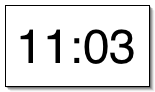
\includegraphics[height=1cm,keepaspectratio]{./figures/cl1} \end{minipage} & \mbox{}\hspace{1cm} & One four-digit display?\\
\mbox{}\\
\begin{minipage}{3cm}
Or two two-digit displays
\end{minipage}& & \begin{minipage}{3cm}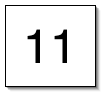
\includegraphics[height=1cm,keepaspectratio]{./figures/cl2}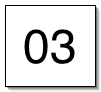
\includegraphics[height=1cm,keepaspectratio]{./figures/cl3}\end{minipage}
\end{tabular}
\end{frame}

\begin{frame}
\begin{itemize}
\item A sensible approach if we go for 2*2-digit displays (`NumberDisplays') is to 

\begin{itemize}
\item write a NumberDisplays class which allows us to show any two digit number (i.e. a template for all NumberDisplays)

\item write a ClockDisplay class that creates two NumberDisplay instances
\item In other words, develop one class 
\item that (in turn) creates two instances of another class (two Objects)
\end{itemize}
\end{itemize}
\end{frame}

\begin{frame}
\frametitle{Class diagram}
\begin{center}
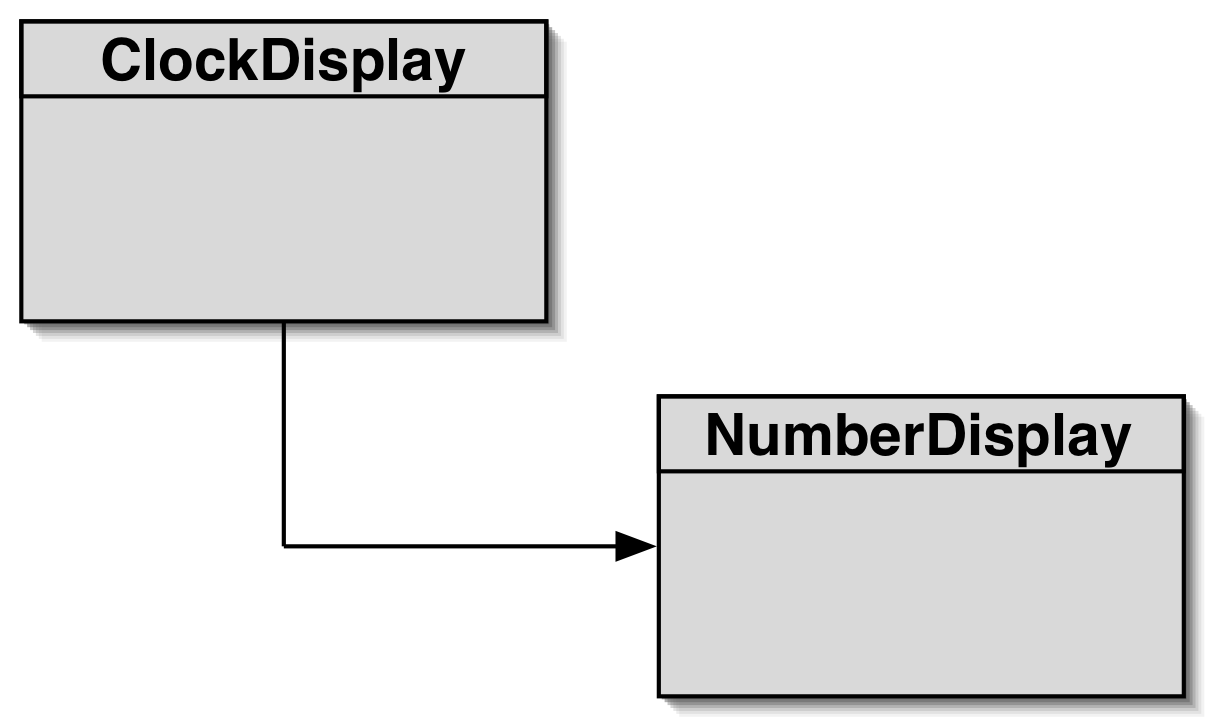
\includegraphics[height=5cm, keepaspectratio]{./figures/class}
\end{center}
\end{frame}

\begin{frame}
\frametitle{Object diagram}
\begin{center}
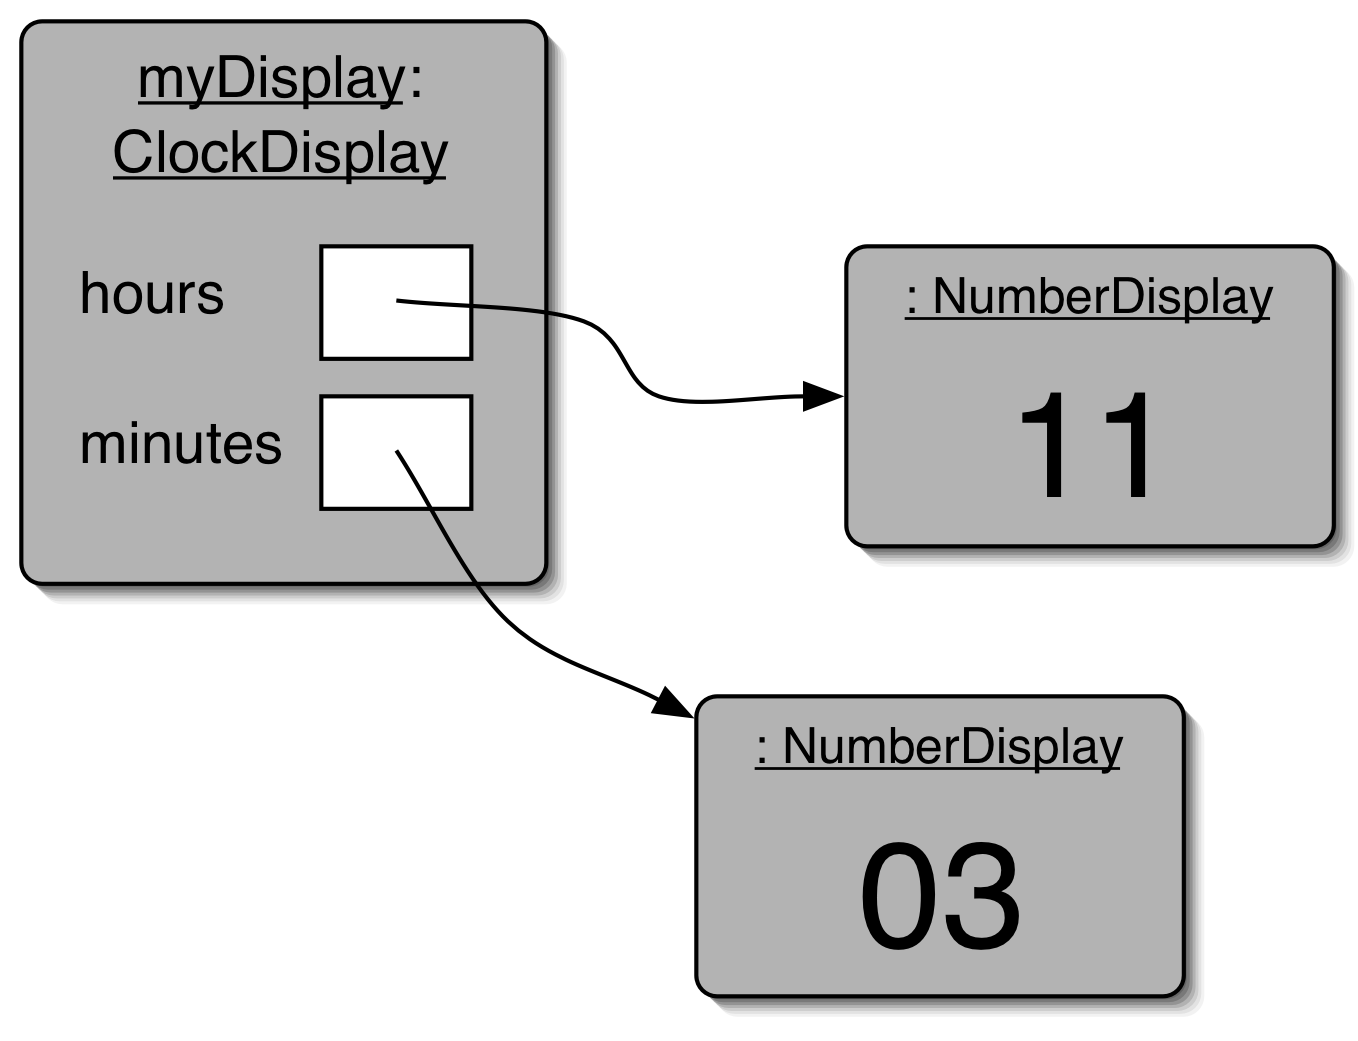
\includegraphics[height=5cm, keepaspectratio]{./figures/object}
\end{center}
\end{frame}

\begin{frame}
\begin{itemize}
\item Class Diagrams

\begin{itemize}
\item Show the classes of an application and the relationships
\item between them
\item Give information about the source code 
\item Static view of the program
\end{itemize}
\item Object Diagrams

\begin{itemize}
\item Show objects and their relationships at one moment in time during the execution of the program 
\item Dynamic view of the program
\end{itemize}
\end{itemize}

\end{frame}

\begin{frame}[fragile]
\frametitle{Implementation: NumberDisplay}
\begin{lstlisting}[linewidth=6cm]
public class NumberDisplay
{
    private int limit;
    private int value;

    Constructor and
    methods omitted.
}
\end{lstlisting}
\end{frame}

\begin{frame}[fragile]
\frametitle{Implementation: ClockDisplay}
\begin{lstlisting}
public class ClockDisplay
{
    private NumberDisplay hours;
    private NumberDisplay minutes;

    Constructor and
    methods omitted.
}
\end{lstlisting}
\end{frame}


\begin{frame}[fragile]

\begin{itemize}
\item We will use the incremental development approach described above:
\item Starting with class comments and a class definition for the NumberDisplay class (no import statements are needed)
\item all  of  the code needed to create a (very basic) DigitalClock will be available on Moodle
\end{itemize}
\end{frame}

\begin{frame}[fragile]
\begin{itemize}
\item But first a few words on Java Strings:
\begin{itemize}
\item Java provides a String class
\item which in turn means that we can use String as a data type
\item Now that we know a little more about the construction of a Java class, we can guess that theString class provides us with at least one constructor
\item in fact it provides us with more than one
\item but the simplest is as follows:
\end{itemize}
\end{itemize}
\end{frame}

\begin{frame}[fragile]
\begin{block}{}
\small
\begin{lstlisting}
public class HelloWorld {

    public static void main(String[] args) {
    	
    	//Call String constructor to create new String
    	String greeting = "HelloWorld";
    	
        System.out.println(greeting);
    }

}

\end{lstlisting}
\end{block}
\end{frame}

\begin{frame}[fragile]
\begin{itemize}
\item The String class also provides us with accessors 
\item e.g. length()
\end{itemize}
\begin{block}{}
\small
\begin{lstlisting}
public class HelloWorld {

    public static void main(String[] args) {
    	
    	String greeting = "HelloWorld";
	int strLength = greeting.length();
    	
        // Concatenates strLength to an emptyString and prints result to the screen
        System.out.println(""+strLength);
    }
}
\end{lstlisting}
\end{block}
\end{frame}

\begin{frame}[fragile]
\begin{itemize}
\item: Note the . notation used to call an accessor method of String greeting
\item: Note also the use of "+" to concatenate strLength to a String
\item: Finally, note the possibility of concatenating ints (or floats or chars) to a String - much easier than C.
\end{itemize}
\end{frame}

\begin{frame}[fragile]
\begin{itemize}
\item the use of + to concatenate Strings is extremely common in java
\item though a more formal concatente() method does exist
\item being able to concatenate any object to a string is also a big help when printing
\item this means that we do not need to use display formatting when printing combinations of Strings and values
\item we can simply print a long concatenation expression (starting with a String)
\end{itemize}
\begin{block}{}
\begin{lstlisting}
public class HelloWorld {

    public static void main(String[] args) {
    
        System.out.println(""+4.0+"Hello"+5);
    }
} 
\end{lstlisting}
\end{block}
\end{frame}

\begin{frame}
\begin{itemize}
\item What is actually happening is that the non String data is being represented in a String before printing
\item using the toString() method that is provided in each class
\item you may not like the way that Java represents data of other types in a String
\item but some representation is always possible. 
\end{itemize}
\end{frame}

\begin{frame}
\begin{itemize}
\item Importantly, however, we cannot change the contents of a Java String once it has been created (Unlike a C String)
\item We cannot, for example, create a String and change the fourth letter.
\item The Java compiler will simply return an error if we try
\end{itemize}
\end{frame}

\begin{frame}
\begin{itemize}
\item We can describe this situation as one in which the Strings class does not provide us with mutator methods
\item Java Strings are, therefore described as \alert{immutable}
\item definition: An \alert{immutable data type} is a type whose state (contents) cannot be changed after creation.
\item defintion: A \alert{mutable} data type is a type whose data members, such as properties, data and fields, can be modified after its creation.
\end{itemize}
\end{frame}

\begin{frame}[fragile]
\begin{itemize}
\item Now we can return to developing a NumberDisplay class
\item following the iterative development approach, we will start with a very simple version of the code
\item i.e. a version which simply defines the class but provides neither fields nor methods
\end{itemize}
\tiny
\begin{block}{}
\begin{lstlisting}
/**
*Add comments describing class here
 */
public class NumberDisplay{
}
\end{lstlisting}
\end{block}

\end{frame}

\begin{frame}[fragile]

\begin{itemize}
\item We can then add a definition of the fields needed by NumberDisplays
\end{itemize}

\begin{block}{}
\begin{lstlisting}
    private int limit;
    private int value;
\end{lstlisting}
\end{block}
\end{frame}

\begin{frame}[fragile]

\begin{itemize}
\item Next, we define constructors for the NumberDisplays
\end{itemize}

\begin{block}{}
\begin{lstlisting}
    /**
     * Constructor for objects of class NumberDisplay
     */
    public NumberDisplay(int rollOverLimit)
    {
        limit = rollOverLimit;
        value = 0;
    }
\end{lstlisting}
\end{block}

\end{frame}

\begin{frame}[fragile]

\begin{itemize}
\item We can also define the Accessors for the Number Display class
\end{itemize}

\scriptsize
\begin{block}{}
\begin{lstlisting}
    /*
     * Return the current value.
     */
    public int getValue()
    {
        return value;
    }
    /*
     * Return current value as a two-digit String. 
     * If value < 10, pad with leading zero.
     */
    public String getDisplayValue()
    {
        if(value < 10)
            return "0" + value;
        else
            return "" + value;
    }
\end{lstlisting}
\end{block}

\end{frame}

\begin{frame}[fragile]

\begin{itemize}
\item ...and finally the mutators
\end{itemize}

\begin{block}{}
\begin{lstlisting}
   /**
     * Set initial value. 
     * If value<0 or over limit, do nothing.
     */
    public void setValue(int replacementValue)
    {
        if((replacementValue >= 0) && (replacementValue < limit))
            value = replacementValue;
    }
    /**
     * Increment the display value by one, 
     * roll over if limit is reached.
     */
    public void increment()
    {
        value = (value + 1) % limit;
    }

\end{lstlisting}
\end{block}

\end{frame}

\begin{frame}

\begin{itemize}
\item Having written code that defines the NumberDisplay class
\item i.e. a template for all NumberDisplay Objects
\item we can now write a ClockDisplay class 
\item That uses two NumberDisplay Objects
\end{itemize}

\end{frame}

\begin{frame}[fragile]

\tiny
\begin{block}{}
\begin{lstlisting}
/*
* Add comments describing ClockDisplay
 */
public class ClockDisplay
{
}
\end{lstlisting}
\end{block}

\end{frame}

\begin{frame}[fragile]
\frametitle{Adding Detail: Fields, Constructors, Mutators, Accessors}
\begin{block}{}
\begin{lstlisting}
    private NumberDisplay hours;
    private NumberDisplay minutes;
    private String displayString;    
\end{lstlisting}
\end{block}

\end{frame}

\begin{frame}[fragile]
\begin{block}{}
\begin{lstlisting}
     /*
     * Constructor for ClockDisplay objects, setting time to 00:00
     */
    public ClockDisplay()
    {
        hours = new NumberDisplay(24);
        minutes = new NumberDisplay(60);
        updateDisplay();
    }
    /*
     * Constructor for ClockDisplay objects, specifying time
     */
    public ClockDisplay(int hour, int minute)
    {
        hours = new NumberDisplay(24);
        minutes = new NumberDisplay(60);
        setTime(hour, minute);
    }
\end{lstlisting}
\end{block}

\end{frame}

\begin{frame}[fragile]
\tiny
\begin{block}{}
\begin{lstlisting}
    /*
     * Mutator that sets time
     */
    public void setTime(int hour, int minute)
    {
        //some code
    }
     /*
     * Mutator that updates clock by one minute every minute
     */
    public void timeTick()
    {
        //some code
    }
\end{lstlisting}
\end{block}

\end{frame}


\begin{frame}[fragile]
\tiny
\begin{block}{}
\begin{lstlisting}
    /*
     * Mutator that updates the internal string that represents the display.
     */
    private void updateDisplay()
    {
        //some code that calls String methods
    }
\end{lstlisting}
\end{block}
\end{frame}

\begin{frame}[fragile]
\tiny
\begin{block}{}
\begin{lstlisting}
     /*
     * Return the current time of this display in the format HH:MM.
     */
    public String getTime()
    {
        //some code
    }
    
    /*
     * Update the internal string that represents the display.
     */
    private void updateDisplay()
    {
        //some code
    }
\end{lstlisting}
\end{block}
\end{frame}

\begin{frame}
\frametitle{Access Modifiers 1}
\begin{itemize}
\item Note: 

Public variables:

\begin{itemize}
\item can be seen (accessed) and changed (mutated) externally
\item i.e. by Objects of this and other classes
\bigskip
\item e.g. private int value; 
\bigskip
\item this usually turns out to be a terrible idea
\item use private variables and accessors/mutators instead
\end{itemize}
\item Private methods

\begin{itemize}
\item private void updateDisplay()
\item can only be called within the Class
\end{itemize}
\end{itemize}
\end{frame}

\begin{frame}
\frametitle{Access Modifiers 2}
\begin{itemize}
\item Note: 

\item Public methods:

\begin{itemize}
\item e.g. public void increment() 
\item can be called externally
\item i.e. by Objects of this and other classes
\bigskip
\item constructors: (Almost) always public
\item mutators: case by case
\item accessors: often public
\end{itemize}
\item Private methods

\begin{itemize}
\item e.g. private void updateDisplay()
\item can only be called within the Class
\end{itemize}
\end{itemize}
\end{frame}

\begin{frame}[fragile]
\begin{itemize}
\item Finally, to start our digital clock, we need a third class containing a main() method, which creates a new ClockDisplay
\item NB we dont need to do any more work to create the NumberDisplays, the ClockDisplay will do that
\end{itemize}
\begin{block}{}
\begin{lstlisting}
public class DigitalClock {

    public static void main(String[] args) {
    	
    	//Call String constructor to create new ClockDisplay
    	ClockDisplay cd = new ClockDisplay();
    	
    }

}
\end{lstlisting}
\end{block}
\end{frame}

\end{document}
